\documentclass[journal]{IEEEtran}
\usepackage{amsmath,amssymb,amsfonts}
\usepackage{tabularx}
\usepackage[utf8]{inputenc} % allow utf-8 input
\usepackage[T1]{fontenc}    % use 8-bit T1 fonts
\usepackage{url}            % simple URL typesetting
\usepackage{booktabs}       % professional-quality tables
\usepackage{amsfonts}       % blackboard math symbols
\usepackage{nicefrac}       % compact symbols for 1/2, etc.
\usepackage{microtype}      % microtypography
\usepackage{graphicx}
\usepackage{float}
\restylefloat{table}
\usepackage{hyperref}
\usepackage{multicol}
\usepackage{caption}
\usepackage{subcaption}
\usepackage{amsmath}
\usepackage{algorithm}
\usepackage{algpseudocode}
\usepackage{tikz}
\usetikzlibrary{trees}
\usepackage{listings}

\DeclareMathOperator*{\argmax}{arg\,max}  % in your preamble
\DeclareMathOperator*{\argmin}{arg\,min}  % in your preamble

\usepackage{textcomp}


%\usepackage[retainorgcmds]{IEEEtrantools}
%\usepackage{bibentry}
\usepackage{xcolor,soul,framed} %,caption

\usepackage[noadjust]{cite}
%\usepackage{biblatex}
%\bibliographystyle{plain}

\usepackage[font=small]{caption}

%=== TITLE & AUTHORS ====================================================================
\begin{document}
\bstctlcite{IEEEexample:BSTcontrol}
    \title{test}
\title{A Control Rearcher's Guide to the Reinforcement Learning Galaxy: A Survey}
\author{ Zongqiang Pang,Liping Bai ~\IEEEmembership{Member,~IEEE,} \thanks{Nanjing Unversity of Posts and Telecommunications, College of Automation \& College of Artificial Intelligence, Nanjing, Jiangsu,210000 China email:zqpang@njupt.edu.cn}}
% ====================================================================
\maketitle
% === ABSTRACT ====================================================================
% =================================================================================
\begin{abstract}
This paper is aimed at providing researchers in the field of control and optimization a bridge for incorporating deep reinforcement learning into their work. We are not talking about the low hanging fruits such as adding visual recognition capacity into the control loops, but technical details on how to take advantage of the progresses brought about by deep learning and its computational infrastructure. Off the shelf implementations of various reinforcement learning agents written in either PyTorch or Tensorflow can be easily found. Yet, when control researchers venture into this subject, they would find out that there is still quite a lot caveats and pitfalls when it comes to applying neural network to optimization problems. They can't just formulate their optimization problem into reinforcement learning setup and let those off the shelf agents have a go at it. In this paper, we present the taxotamy of reinforcement learning from the perspective of optimization and we tease out the most important concepts while screening away ideas that might be relevent to other field yet less so for control. We hope to provide control researchers roadmap as of how to further their research by riding the wave of reinforcement learning.
\end{abstract}
% === KEYWORDS ====================================================================
% =================================================================================
\begin{IEEEkeywords}
Reinforcement Learning, Control Theory, Optimal Control, Optimization
\end{IEEEkeywords}
% For peer review papers, you can put extra information on the cover
% page as needed:
 %\ifCLASSOPTIONpeerreview
 %\begin{center} \bfseries EDICS Category: 3-BBND \end{center}
% \fi
%
% For peerreview papers, this IEEEtran command inserts a page break and
% creates the second title. It will be ignored for other modes.
\IEEEpeerreviewmaketitle


% === I. Paper =============================================================
% =================================================================================
\section{Introduction}
\IEEEPARstart{R}{einforcement} learning is the process of methotically extracting information from observations to gradually bound the policy distribution, either directly through policy gradient methods or via scaffolding measurements, maximizing the expected reward along a trajectory. This objective is quite similar to that of Trajectory Optimization which utilizes myriade of computational techniques to incorporating scripted constraints, which capture the dynamics of a system with exquisit differential equations, to carve out the optimal trajectories. The theoretical foundation of reinforcement learning are statistical learning theory and dynamic programming. When the first batch of reasonable RL results were introduced, they were met with coldness. The preface of Bertseka's book Neuro Dynamic Programming provides a good sample on reinforcement learning is perceived by the control community back then: ...These methods (Reinforcement Learning) were aiming to provide effective suboptimal solutions to complex problems of planning and sequential decision making under uncertainty, that for a long time were thought to be intractable. Our first impression was that the new methods were ambitious, overly optimistic, and lacked firm foundation....Three years later, after a lot of study, analysis, and experimentation, we believe that our initial impressions were largely correct. \cite{Bertsekas1996NeuroDynamicP}

Yet today, scores of control theoriest can't wait to incorporate reinforcement learning into their research. What has changed is not the theoretical foundation of RL but its computational infrastructure. Before 2010, the predominent methods used for function approximation are various forms kernel methods, where feature spaces are transformed such that linear compuational techniques can be utilized. Today, the default function approximator are neural networks. Another major change in computation is that of GPU. Before the advent of CUDA, GPU programming requires PhD in computer graphics. Today, anyone who is proficient in C/C++ can programme GPU to parallelize their compuation. This capacity sometimes brought about unexpected result. For instance, the asymchronous actor critic method is not exactly rigirous mathematically speaking, yet with fast parallelized computation, it works in reality.

Therefore, the difficulty facing control theoriest is not the theories behind RL, but the computational details. In our paper, we want to provide control researchers with the most up-to-date version of the compuations, which can be different from the cananical versions you see in RL textbooks.



Respectively, they are the "Black Box" and "White Box" approach to the problem of control, neither is perfect. The "Black Box" approach requires copious amount of data. Efforts has been made to make it more broadly applicable and more efficient. For instance, imitation learning and reverse reinforcemnt learning \cite{Ho2016GenerativeAI} aims at automatically derive constraints from observed best solution; Sergey Levine utilizes unsupervised learning to build an agent with intuitions of the physical world \cite{Finn2016UnsupervisedLF}; Chelsea Finn introduced Meta-Learning \cite{Finn2017ModelAgnosticMF} to extract overaching structures embedded in similar tasks of different setting. This is a very active area of research, mostly done by computer scientists who are traiend in statistical learning theory. Meanwhile, despite efforts from the best mathematical minds, some complicated dynamics still elude the "White Box" approach.

It is obvious that biological entities approaches control from both angles. We have some inkling of how a system might work and how our actions would affect that system and we can learn to control it via trial and error. Yet, unfortunately, these two subjects are studied by two communities of researchers who use different notations to discribe the same processes and they publish their researches only in journals of their own disciplines. In this paper, we hope to provide a bridge for researchers in the field of control who would like to incorporate reinforcement learning into their works.

We are not the first ones to take up this challenge. Recently, there are interdiscipline conferences held specifially for the purpose of briding the gaps between these groups of people, for instance the \href{https://l4dc.mit.edu/}{L4DC (Learning for Dynamic Control) conference} and \href{https://www.ipam.ucla.edu/programs/workshops/intersections-between-control-learning-and-optimization/}{Intersections between Control, Learning and Optimization Workshop}.

In this paper, we build on the work of Benjamin Recht \cite{Recht2018ATO} to formulate reinforcelent learning in the language of optimization. The first task facing control researchers is to consolidate the notation between control and reinforcement learning communities. Control communities use the notation system introduced by Lev Pontryagin. State is denoted $ \mathcal{X}$, Action is denoted $\mathcal{U}$, which is the first letter of Russian for "Action", the dynamics and stocasticity is captured by physical model constraints $x_{t+1}=f(x_t,u_t,e_t)$ where e denote the noise of a system. The objective is usually to minimize the cost funtion $\mathcal{J(.)}$. Reinforcement Learning communities use the notation system introduced by Richard Bellman who studied dynamic programming. State is denoted $\mathcal{S}$, Action is denoted $\mathcal{A}$. The dynamics and stochaticity is captured via transition matrix $\mathcal{P}$ of a Markov Decision Process.The objective of RL is to maximize the reward function $\mathcal{R(.)}$. Yet, if we set the transition matrix to be identical to the noise, then it is clear that the underlying process behind these two notation system are exactly the same. The differences are nothing but style. Since the audience of our paper is the control community, we would cast reinforcement learning in the control notation system.

We would first introduce where to bring approximation into optimization. We then elaborate on the enumerated path in section II and list all the key papers in this area of research. In section VI, we introduce other methods such as distributed and multiagent formulation of optimization problems to better take advantage of the computational infrastructure for control problems.
% === II. Harmonically-Terminated Power Rectifier Analysis ========================
% =================================================================================
\section{Where to Approximate}
Reinforcement Learning is not a new subject, control researchers probably know it by the name Approximate Dynamic Programming. The renewed interest in this area is the result of progressed made in Deep Learning, which brought the potential of neural network as a universal approximator \cite{Hornik1991ApproximationCO} to fruition. When reinforcement learning is armed with enhanced approximating capacity, we finally get a glimpse into what this line of research can do. AlphaGo, AlphaStar, just name a few.

Broadly speaking, there are three avenues where neural network based approximation can find its way into optimization as shown in \ref{fig:1}. One is learning a dynamics model from sample; Second is policy gradient based learning; Third is approximation of cost to go functions such as value funtion and Q function. The details of the implementation would be specified in the subsequent sections.

\begin{figure}[H]
    \centering
    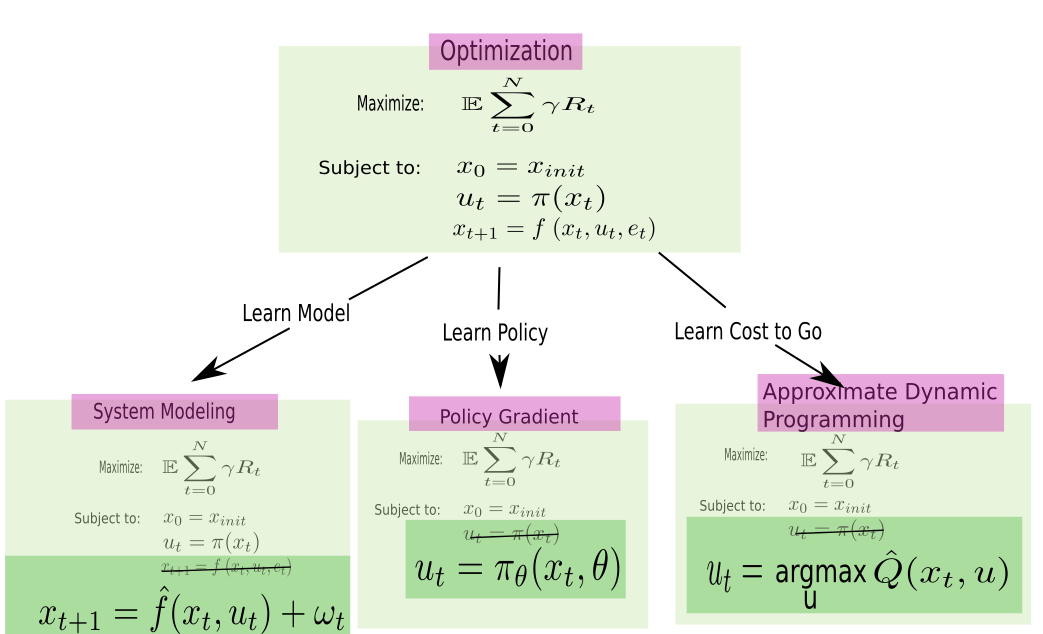
\includegraphics[width=0.5\textwidth]{Control.png}
    \caption{From Optimization to Learning}
    \label{fig:1}
\end{figure}
<<<<<<< HEAD

The trajectory construction process itched in control researchers mind is that ev

The constraints imposed in the Trajectory Optimization formulation manifest themselves directly in policy $\pi(x)$ and resulting in either a narrow band of trajectories or a single optimal solution. However, adjustments in the reinforecement learning formuation is not the policy per se but its distribution. Eventually, what we hope to acheive via learning is a policy distribution, either through policy gradient method or cost to go method, which would maximize the expected reward of a trajectory.

\section{How to Approximate}
Before 2010, most techniques offered in statistical learning theory are that of kernel methods.
















=======
TEST
>>>>>>> 0a11db63e0e342d29b408b28c28e9214f7e293e2
Before we dive into the detailed researches in each category, we'd like to introduce additional mathematical tools and measurements that has been proven useful in merging reinforcement learning with optimization. One of the most important change of perspectives when control researchers ventures into the land of reinforcement learning is to formulate optimization as an inference problem \cite{Levine2018ReinforcementLA}. Tranditional optimization would translate constraints imposed on the struture into definitive trajectories, subject to disturbance and correction. Yet inference view of optimization is an ever narrowing band od distribution as information trickles in via experiments.

There are two things control researchers should be aware of. One, if you simply apply reinforcement learning as it is written in Richard Sutton's book, it probably won't work for you. Additional statistical learning techniques are required. Two, Statistical learning is booming with ideas at this point. Every newly invented measurement and methods could be pretzeled into a self-sustainly structure if you know how to make such arguments, that does not mean it would be a useful tool for your research.

Here we point out two concepts: Mutual Information and Baysian NeuroNet, which have proven to be integral for converting optimization into an inference.



The intuition behind maximum entropy reinforcenement learning is the heuristic that when we don't know all the circumstance, we should prioritize options that could give us more choices regardless of how the system dynamics turns out to be. Statitically speaking, this means we should maximize the entropy of a distribution, which measures how uncertain or how broad the distributionb is.

The mathematical measurement used is mutual information \cite{Kullback1951ONIA}. It measures how much information regarding the random variable X is contained in the distribution of random variable Y. A reasonable question to ask is that out of all those measurements which captures "distance" in meansurement theory, why a divergence is chosen? Turns out, this choice is made because of its computational convenience, much like exponentials are chosen in integral transform because its nice features.



\section{System Modelling}

There are two ways for collecting data of the system. One is offline. Just collecting as much trajectories as possible about this system and then build the model later. Second is online data collection where a sample is collected and then incorporated into the model building process right away.

Strictly speaking, offline data collection based model building belongs to the domain of System Identification rather than reinforcement learning. But since it is tangentially related to our paper, we still list it here. After the data is collected and a system model is trained from offline data, an appropriate controllers can be computed based on that model. There are numerous applications in this line of research, supposedly the first successfully implemented non-linear controller based on this method is that of Caltech's Neural Lander. \cite{Shi2019NeuralLS}

The online data collection and training method goes under the name iteration learning based model predictive control (ILMPC).This model training process doesn't have to start from scratch, althought that is certainly an option. Most likely there already exist a model that partially describes the system. It would be more efficient if we can somehow combine that partial model with a neural network, which would capture the unmodelled dynamics via online training.

A existing model can be additively combined \cite{Hewing2020LearningBasedMP} with a neural network, or it can be embedded into a neural network \cite{Mohan2020EmbeddingHP} as shown by Fig. \ref{fig:combine}. Optimization solver can also be embedded in the neural network as a laywer to encourage faster convergence. \cite{BelbutePeres2018EndtoEndDP} \cite{BelbutePeres2020CombiningDP} \cite{Agrawal2019DifferentiableCO}.

\begin{figure}[H]
\centering
\begin{subfigure}{0.25\textwidth}
  \centering
  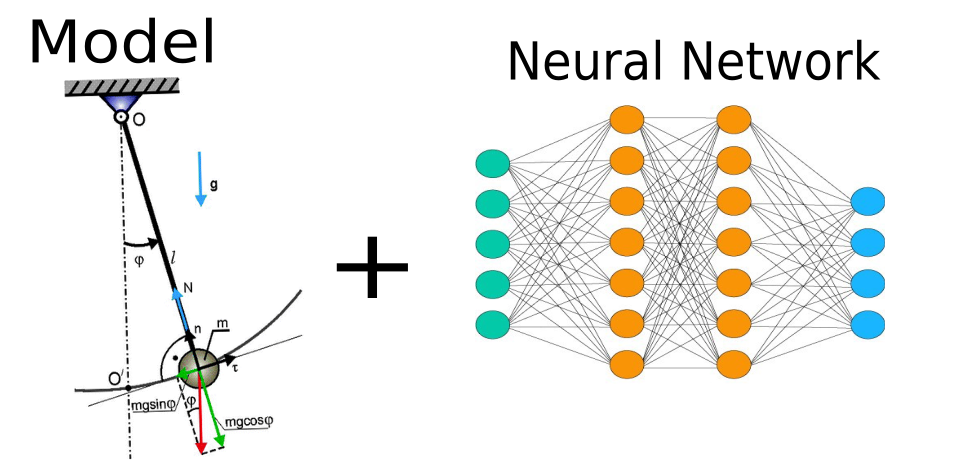
\includegraphics[width=\linewidth]{combine1.png}
  \caption{Additive}
\end{subfigure}%
\begin{subfigure}{.25\textwidth}
  \centering
  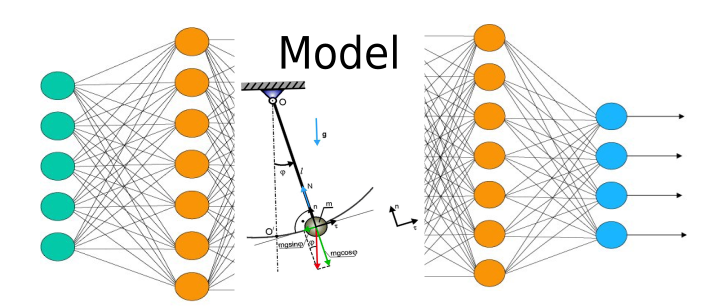
\includegraphics[width=\linewidth]{combine2.png}
  \caption{Embedding}
\end{subfigure}
\caption{Combine Model and Neural Net}
\label{fig:combine}
\end{figure}


While in theory the aforementioned modelling method should work, in practice it is proven to be far from optimal.  \cite{8463189}. One possible explanation is that any overfitting of the model along the way would be difficult to overcome by subsequent training, resulting in suboptimal performance. One solution is to measure uncertainly of the model with Bayesian Neural Network.

The venena formulation of neuronetwork is one where the weight of each neuron $w_i$ is a single number, which is adjusted based on the backward propogation process. Baysian Neural Network(BNN) is a network where the weigh is subject to a parameterized distribution as shown in Fig. \ref{fig:2}
\begin{figure}[H]
    \centering
    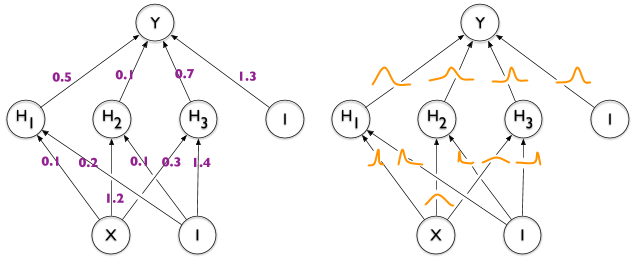
\includegraphics[width=0.3\textwidth]{bnn.png}
    \caption{Neural Network and BNN}
    \label{fig:2}
\end{figure}


BNN is used to measure the uncertainly of the model and avoid overfitting. For exact method, please refer to these papers. \cite{Blundell2015WeightUI} \cite{Gal2017ConcreteD}

\section{Policy Gradient}
The collected data can be used to train a model which informs which actions should be chosen. It can also be used to train the policy distribution either directly or through policy gradient. The direct policy training method is a theoretical possibility, but due since the number of actions along a trajectory is usually rather large, the valishing gradient problem facing this methods makes it had to implement. In this paper,we focus our discussion on the Policy Gradient Method.

The policy is modelled with parameterized distribution, samples collected based on that policy. Based on how well the trajectories pan out, we adjust policy parameters to make the better choices more likely. The classical Policy Gradient based method is called REINFORCE and can be found in this paper: Simple statistical gradient-following algorithms for connectionist reinforcement learning: introduces REINFORCE algorithm. \cite{Williams1992SimpleSG}. When control researchers are first exposed to the proof of policy gradient method provided in Richard Sutton's book, they would find it difficult to swallow. The notations are tidious and the logic non-rigirous. A more rigirous proof was only recently presented, please see this paper for rigirous proof of policy gradient method. \cite{Schulman2015TrustRP}

Policy Gradient is one of the core component of reinforcement learning, yet as would refrain from list the important papers for now since most of modern implementation of policy gradient method is used in tanden with methods we are going to introduce in the next section to construct some sort of bootstrap structure for variance reduction.

\section{Approximate Dynamic Programming}
Control theoriests are familiar with Approximate Dynamic Programming, it 






\subsection{Value Iteration and Policy Iteration}
\subsection{Maximum Entropy Reinforcement Learning}

The go to text book for reinforcement learning community is that of Richard Sutton \cite{Sutton1998IntroductionTR}. In the system contstructed by Richard, the objective of an agent is to maximize discounted reward. This formulation is proven a sound goal in the context of video games. However, for optimizations with a physics underpining, reward maximization is not adequate since noise and disturbances is common place in control.

Exploration and Exploitation trade off is something studied exhaustively in the reinforcement learning community. A common strategy is $\epsilon$ greedy policy where the value of epsilon decays as the learning progresses. Yet, the decaying rate is a hyperparater that need to be tuned. Is there are more sysmtmatical way to balance the exploration and exploitation trade-off? This is particularly important for control related training since this application has considerable amount of disturbance and noise. If the policy converges too soon, any subsequent disturce can deviate the trajectory to the extend that it is no longer controllable.



\section{Other Ways to Utilize Increased Computational Power}
\subsection{Multiagent Formulation}



\subsection{Random Shoot}
One of the corrilary of the development of reinforcement leraning is improvement in computational infrastructure, which is something the control community can take advantage of. Before this wave of hype in machine learning, GPU enabled computation was a specialty knowledge that is only accessable to large corporations. But now, with CUDA and related software, such compuational power is as easy

Random shoot is the idea if rolling out trajectory at random and wht the fuck is random shoot?




\bibliographystyle{IEEEtran}
\bibliography{Bibliography}
%\printbibliography



\end{document}
